%%%%%%%%%%%%%%%%%%%%%%%%%%%%%%%%%%%%%%%%%
% Stylish Article
% LaTeX Template
% Version 2.1 (1/10/15)
%
% This template has been downloaded from:
% http://www.LaTeXTemplates.com
%
% Original author:
% Mathias Legrand (legrand.mathias@gmail.com) 
% With extensive modifications by:
% Vel (vel@latextemplates.com)
%
% License:
% CC BY-NC-SA 3.0 (http://creativecommons.org/licenses/by-nc-sa/3.0/)
%
%%%%%%%%%%%%%%%%%%%%%%%%%%%%%%%%%%%%%%%%%

%----------------------------------------------------------------------------------------
%	PACKAGES AND OTHER DOCUMENT CONFIGURATIONS
%----------------------------------------------------------------------------------------

\documentclass[fleqn,10pt]{SelfArx} % Document font size and equations flushed left

\usepackage[frenchb]{babel} % Specify a different language here - english by default
\usepackage[utf8]{inputenc}
\usepackage{xspace}
\usepackage{multirow}
\usepackage{subfig}
\usepackage{amsmath}

%----------------------------------------------------------------------------------------
%	COLUMNS
%----------------------------------------------------------------------------------------

\setlength{\columnsep}{0.55cm} % Distance between the two columns of text
\setlength{\fboxrule}{0.75pt} % Width of the border around the abstract

%----------------------------------------------------------------------------------------
%	COLORS
%----------------------------------------------------------------------------------------

\definecolor{color1}{RGB}{0,0,90} % Color of the article title and sections
\definecolor{color2}{RGB}{0,20,20} % Color of the boxes behind the abstract and headings

%----------------------------------------------------------------------------------------
%   MACROS
%----------------------------------------------------------------------------------------
\newcommand{\bcom}{b$\textless\textgreater$com\xspace}
\newcommand{\T}{T(x, y, t_{0})}
\newcommand{\Gx}{G_{x}(x,y,t_{0})}
\newcommand{\Gy}{G_{y}(x,y,t_{0})}

%----------------------------------------------------------------------------------------
%	HYPERLINKS
%----------------------------------------------------------------------------------------

\usepackage{hyperref} % Required for hyperlinks
\hypersetup{hidelinks,colorlinks,breaklinks=true,urlcolor=color2,citecolor=color1,linkcolor=color1,bookmarksopen=false,pdftitle={Conversion HFR LFR},pdfauthor={Florent GUIOTTE, Paul LE DENN, Brieuc DANIEL, Danchi LI}}

%----------------------------------------------------------------------------------------
%	ARTICLE INFORMATION
%----------------------------------------------------------------------------------------

\JournalInfo{Projets Industriels, \bcom, ESIR, 2016} % Journal information
\Archive{Article technique de restitution} % Additional notes (e.g. copyright, DOI, review/research article)

\PaperTitle{Conversion HFR LFR} % Article title

\Authors{Florent GUIOTTE\textsuperscript{1}, Paul LE DENN\textsuperscript{1}, Brieuc DANIEL\textsuperscript{1}, Danchi LI\textsuperscript{1}\\Olivier LE MEUR\textsuperscript{2}\\Jean-Yves AUBIE\textsuperscript{3}} % Authors

\affiliation{\textsuperscript{1}\textit{Imagerie Numérique, École Supérieure d'Ingénieurs de Rennes, Université de Rennes 1, France\\}
\textsuperscript{2}\textit{École Supérieure d'Ingénieurs de Rennes, Université de Rennes 1, France\\}
\textsuperscript{3}\textit{\bcom, Rennes, France}
} % Author affiliation

\Keywords{Haute fréquence d'image (High Frame Rate, HFR), faible fréquence d'image (Low Frame Rate, LFR), flot optique, conversion} % Keywords - if you don't want any simply remove all the text between the curly brackets
\newcommand{\keywordname}{Mots-Clés} % Defines the keywords heading name

%----------------------------------------------------------------------------------------
%	ABSTRACT
%----------------------------------------------------------------------------------------

\Abstract{Le monde de la vidéo a vu naître de nombreux formats durant ces dernières années. Les technologies ont rapidement évoluée et nous permettent de visionner des vidéos en HD, Full HD et même Ultra HD. 
De la même manière, les cameras permettent de filmer des séquences vidéo HFR avec un rythme d'image de l'ordre de 100 images par seconde — plus fluides que des vidéos LFR — 50 images par secondes. 
Malheureusement, tous les écrans ne sont pas en mesure d'afficher des vidéos enregistrées à de telles fréquences.
Nous travaillons en partenariat avec \bcom pour effectuer la conversion d'une fréquence élevée vers une fréquence adaptée, afin d'obtenir des vidéos compatibles pour tous les écrans.
Une vidéo HFR contient des images plus nettes qu'une vidéo LFR, supprimer une image sur deux provoquerait donc des saccades désagréables à l'œil.
Nous proposons dans notre solution une approche perfectionnée prenant en compte l'effet de flou provoqué par des objets en mouvement.
Cet effet est naturellement présent dans les vidéos LFR et est appelé flou de mouvement ou flou cinétique.
Nous détectons le mouvement dans la vidéo via le calcul d'un flot optique et d'un gradient temporel, puis nous appliquons un traitement pour reproduire le flou cinétique selon le mouvement.\\

The world of video has produced many formats in recent years. Technology has advanced rapidly and allow us to watch videos in HD, Full HD and even Ultra HD.
Similarly, the cameras used to record HFR videos with an image rate of about 100 frames per second — more fluid than LFR video — 50 frames per second.
Unfortunately, all the screens are not able to display these videos recorded at such frequencies.
We partner with \bcom to convert a high frequency to a suitable frequency, in order to get compatible videos for all screens.
A video contains sharper HFR images than LFR video, delete an image on two jerks therefore cause unpleasant to the eye.
We offer our solution in a sophisticated approach taking into account the blur caused by moving objects.
This effect is naturally present in LFR and videos is called motion blur.
We detect motion in the video through calculating an optical flow and a temporal gradient, then apply a treatment to reproduce the motion blur according to the movement.}

%----------------------------------------------------------------------------------------

\begin{document}

\flushbottom % Makes all text pages the same height

\maketitle % Print the title and abstract box

\tableofcontents % Print the contents section

\thispagestyle{empty} % Removes page numbering from the first page

%----------------------------------------------------------------------------------------
%	ARTICLE CONTENTS
%----------------------------------------------------------------------------------------
%\newpage
\section*{Introduction} % The \section*{} command stops section numbering
\addcontentsline{toc}{section}{Introduction} % Adds this section to the table of contents

Les entreprises évoluant dans le domaine du traitement d'image et de la compression vidéo cherchent à développer de nouveaux formats permettant un gain de qualité.
Pour cela, deux paramètres peuvent être améliorés : la qualité spatiale (résolution d'image, compression) et temporelle (haute fréquence d'image).
Ces deux paramètres sont l'objet de travaux au sein de l'institut de recherche technologique \bcom qui a pour objectif de fournir une meilleure sensation d'immersion des spectateurs dans les contenus audiovisuels.
Cet institut de recherche possède un laboratoire étudiant le réalisme des contenus.
Leur but est de développer des outils visant a faciliter la prise en main de ces futurs formats par les professionnels du secteur (cinéma, télévision, jeux, publicité, etc.) et, a terme, par le public.
Parallèlement, les chercheurs de \bcom travaillent sur la possibilité de rendre ces formats lisibles sur des moniteurs non compatibles.
C'est notamment le cas des vidéos enregistrées à une fréquence d'images élevées, typiquement 100 ou 120 images par seconde (ips), non lisibles sur des écrans qui ne peuvent afficher que 50 ou 60 ips maximum.
Dans cette optique, nous sommes amenés à proposer une solution permettant de réduire de moitié la fréquence d'image de vidéos HFR sans détériorer la fluidité des mouvements pour le spectateur.
En HFR, l'intervalle de temps entre 2 images consécutives est très court, les déplacements des objets entre les 2 images le sont donc également.
La succession des images donne alors une impression de mouvement très proche de la réalité.
En LFR, cet intervalle de temps étant plus important, la fluidité est obtenue par un rendu plus flou des objets en mouvements (figure 1). Il s'agit du flou cinétique, provoqué par le temps de pose plus long de la camera lors de la capture d'une image.
Pour réduire la fréquence d'image, la solution intuitive consisterait a supprimer une image sur deux. Néanmoins, des travaux réalises auparavant à \bcom ont montré que cette solution n'est pas satisfaisante car elle ne permet pas de retrouver le flou cinétique.
La vidéo semble alors très hachée.
De même, des traitements globaux comme une combinaison linéaire classique d'images successives n'élimine pas suffisamment les saccades.
Dans ce document, nous étudions la manière dont il est possible de simuler le flou cinétique localement sur les images.
Les deux solutions que nous proposons se basent sur l'estimation du mouvement dans la vidéo originale.
La première consiste à reprendre l'idée d'une combinaison de plusieurs images, cette fois avec une accélération matérielle.
La seconde méthode est l'application de flous cinétiques sur les objets qui se déplacent grâce à des gradient temporels.

%------------------------------------------------

\section{Méthodes}

\subsection{Les méthodes utilisées}

\subsubsection{La décimation simple}
Ici le but est très naïf, il s'agit simplement de supprimer du flux initial une image sur deux et ainsi passer d'un contenu ayant 120 images par seconde à un contenu n'en possédant que 60.

Ce qui a l'avantage d'être le plus rapide à l'exécution mais en contrepartie aucun traitement n'est effectué comme du flou de mouvements.

\subsubsection{La pondération simple}
La pondération simple est le fait de se baser deux images consécutives pour en créer une nouvelle, on s'appuie sur la somme pondérée de deux tableaux multidimensionnels (les canaux étant traités séparément) représentants les deux images en entrée pour ensuite avoir un résultat pondéré à cinquante pour-cent de chaque image.

Ceci a l'avantage de bien représenter la continuité spatiale de deux images proches en plus de diminuer par deux le flux d'images initial.

\subsubsection{La double pondération}
La double pondération quand à elle se base sur trois images consécutives afin de créer notre nouvelle image, ici on s'appuie sur trois sommes pondérées consécutives entre, respectivement, notre image courante et notre image précédente, notre image courante et notre image suivante et finalement la somme pondérée entre ces deux résultats précédents.

Ceci a l'avantage de mieux représenter la continuité spatiale d'images proches en plus de, elle aussi, diminuer par deux le flux d'images initial. Mais elle ne prend pas en compte la compensation de mouvements malheureusement.w

%\include{gradient tst}
\subsubsection{Gradient spatio temporel}
L'une des méthode testée pour générer du flou de mouvement est l'approximation du flot optique à l'aide
d'un gradient spatio temporel.
% TODO: expliquer le flot optique
Cette solution se veut peu coûteuse en calcul, contrairement à la méthode proposée l'année
dernière\cite{hfr2lfr2015} basé sur une extension polynomiale\cite{farneback2003} qui permet
de déterminer précisément le flot optique.

En prenant un flux vidéo, le principe est de générer un gradient en prenant en compte l'image précédente et
l'image suivante, d'où ma notion temporel, en plus du spatial d'un gradient classique.

Nous utiliserons les notations suivantes~:
\begin{itemize}
    \item $I$ : la vidéo, une succession d'image tel que $I : \Omega \in \mathbb{R}^{3} \to \mathbb{R}^{3} $
    \item $I(x, y, t)$ : le pixel de coordonnée $(x, y)$ de l'image $t$ de la vidéo
    \item $G$ : le gradient tel que $ G : \Omega \in \mathbb{R}^{3} \to \mathbb{R}^{2} $.

\end{itemize}

$G(x, y, t)$ représente le vecteur gradient associé au pixel de coordonnée $(x, y)$ de l'image $t$.
On décompose le gradient dans les deux directions~:
% Temporel

\[G(x,y,t) = 
    \begin{bmatrix}
        G_{x}(x,y,t) \\
        G_{y}(x,y,t)
    \end{bmatrix}
\]

Où $G_{x}$ représente le gradient en $x$ et $G_{y}$ le gradient en $y$, semblable à un gradient classique, 
ce qui permet de prendre en compte l'espace.

Par soucis de lisibilité, on utilise $t$ pour symboliser l'emplacement relatif dans le flux d'image, où $t_{0}$ représente donc
l'image actuelle, $t_{-1}$ l'image précédente et $t_{+1}$ l'image suivante.

Dans un premier temps, on utilise un calcul simple du gradient~:
\[
    \begin{cases}
        G_{x}(x,y,t_{0}) = I(x_{-1}, y, t_{-1}) - I(x_{+1}, y, t_{+1}) \\
        G_{y}(x,y,t_{0}) = I(x, y_{-1}, t_{-1}) - I(x, y_{+1}, t_{+1}) \\
    \end{cases}
\]
où on effectue une différence entre le pixel précédent en $x$ ou $y$ entre l'image suivante et l'image
précédente. On obtient les contours des objets et des zones de mouvements.
% TODO: images démo ?

Dans un deuxième temps, afin d'augmenter la robustesse de cet opérateur de gradient,
notre solution implémente un filtre de Sobel adapté à notre utilisation temporel.
Le filtre de Sobel par rapport à la première solution a un rôle de filtre passe bas pour limiter 
l'influence du bruit contenu dans la séquence vidéo sur notre estimation de mouvement~:

\[
    %\begin{bmatrix}
    %    -1 & 0 & 1 \\
    %    -2 & 0 & 2 \\
    %    -1 & 0 & 1 
    %\end{bmatrix}
    \begin{cases}
        G_{x}(x,y,t_{0}) = \\
        \begin{bmatrix}
            I(x^{-1}, y^{-1}, t_{-1}) & I(x_{-1}, y, t_{-1}) & I(x^{-1}, y^{+1}, t_{-1}) \\
            0 & 0 & 0 \\
            I(x^{+1}, y^{-1}, t_{+1}) & I(x_{+1}, y, t_{+1}) & I(x^{+1}, y^{+1}, t_{+1}) \\
        \end{bmatrix} \\
        G_{y}(x,y,t_{0}) = 
        \begin{bmatrix}
                     I(x_{-1}, y_{-1}, t_{-1}) & 0 &          I(x_{-1}, y_{+1}, t_{+1}) \\
            2 \times I(x,      y_{-1}, t_{-1}) & 0 & 2 \times I(x,      y_{+1}, t_{+1}) \\
                     I(x_{+1}, y_{-1}, t_{-1}) & 0 &          I(x_{+1}, y_{+1}, t_{+1}) \\
        \end{bmatrix}
    \end{cases}
\]

On calcule le tenseur de structure associé à notre gradient précédemment obtenus tel que~:
\[
    T(x, y, t_{0}) = 
    \begin{bmatrix}
        G_{x}(x,y,t_{0})^{2} & G_{x}(x,y,t_{0})G_{y}(x,y,t_{0}) \\
        G_{y}(x,y,t_{0})G_{x}(x,y,t_{0}) & G_{y}(x,y,t_{0})^{2} \\
    \end{bmatrix}
\]
Les vecteurs propres et les valeurs propres de ce tenseur permettent d'obtenir rapidement la direction normale
au gradient et une information locale sur l'activité spatio-temporelle de la zone. Par extension, la direction du déplacement et sa vitesse.

Concernant la direction normale au gradient, on l'obtiens avec cette relation\footnote{La notation $\T_{m,n}$
représente le scalaire contenu dans la matrice $\T$ à la ligne $m$ et la colonne $n$.}~:
\[
    \Theta^{+} = 
    \begin{bmatrix}
        2 \times \T_{1,2} \\
        \T_{2,2} - \T_{1,1} + \sqrt{\Delta}
    \end{bmatrix}
    %\begin{bmatrix}
    %    2 \times \Gx \Gy \\
    %    \T_{2,2} - \T_{1,1} + \sqrt{\Delta}
    %\end{bmatrix}
\]
Où~:
\[
    \Delta = (\T_{1,1} - \T_{2,2})^{2} + 4 \T_{1,2}^{2}
\]

Et pour obtenir la cohérence norme, qui permet de détecter les gradients forts~:
\[
    C = \left(\frac{\lambda_{+} - \lambda_{-}}{\lambda_{+} + \lambda_{-}}\right)
\]
Où~:
\[
    \lambda_{\pm} = \frac{\T_{1,1} + \T_{2,2} \pm \sqrt{\Delta}}{2}
\]

La combinaison de la normale au gradient et sa cohérence norme sur l'image entière nous donne un champ 
dense de vecteurs, ou le flux optique.

Pour visualiser ce flux optique, nous avons convertit ces données en image {\em Hue,
Saturation, Lightness (HSL)}~:
\begin{itemize}
    \item La direction est traduite en couleur sur le disque du Hue
    \item La norme est exprimée en luminosité
\end{itemize}

Un exemple de cette visualisation par image HSL est visible figure \ref{hsl}.
\begin{figure}[!ht]%htp]
    \centering
    \subfloat[Image précédente]{\label{hsl:prev}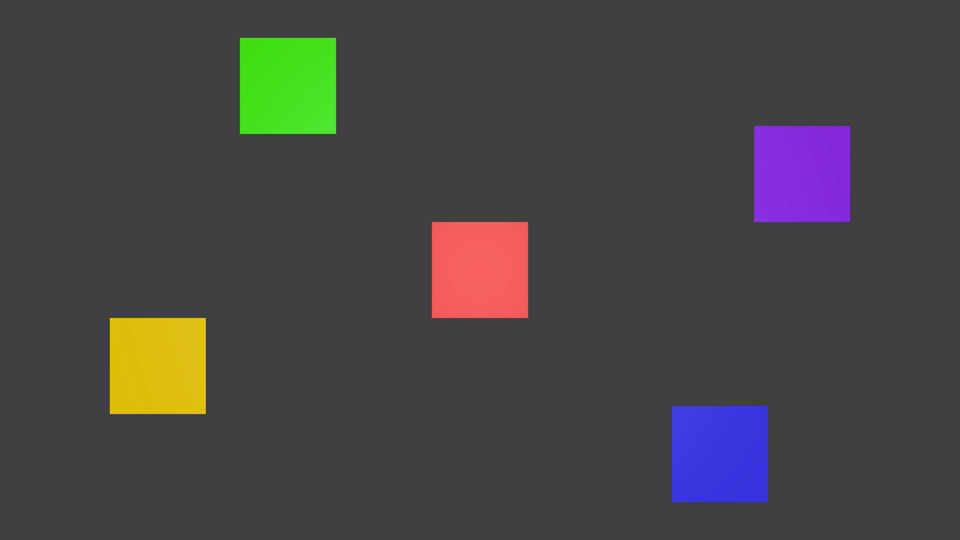
\includegraphics[width=0.5\textwidth]{img/prev.png}}
    \hspace{0.030\textwidth}
    \subfloat[Image suivante]{\label{hsl:next}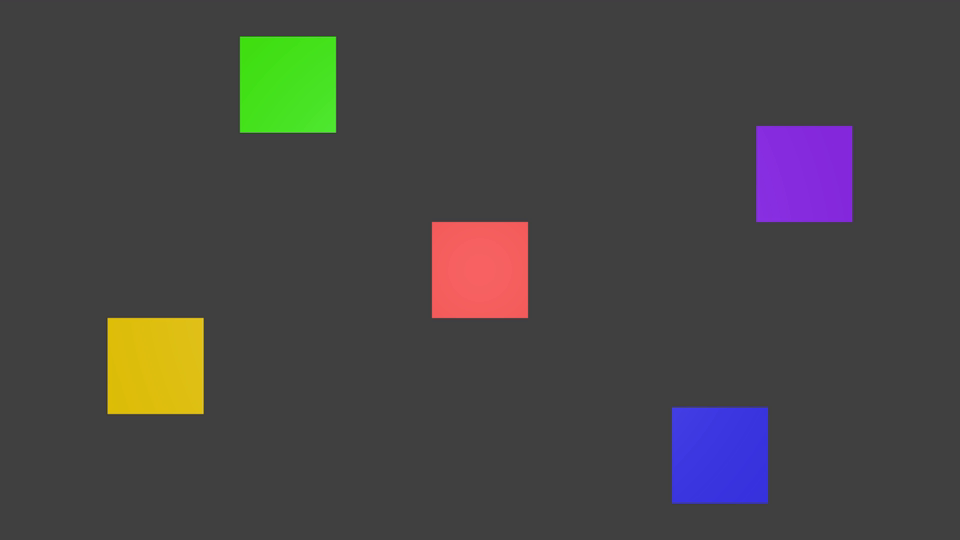
\includegraphics[width=0.5\textwidth]{img/next.png}}
    \hspace{0.030\textwidth}
    \subfloat[Image HSL]{\label{hsl:final}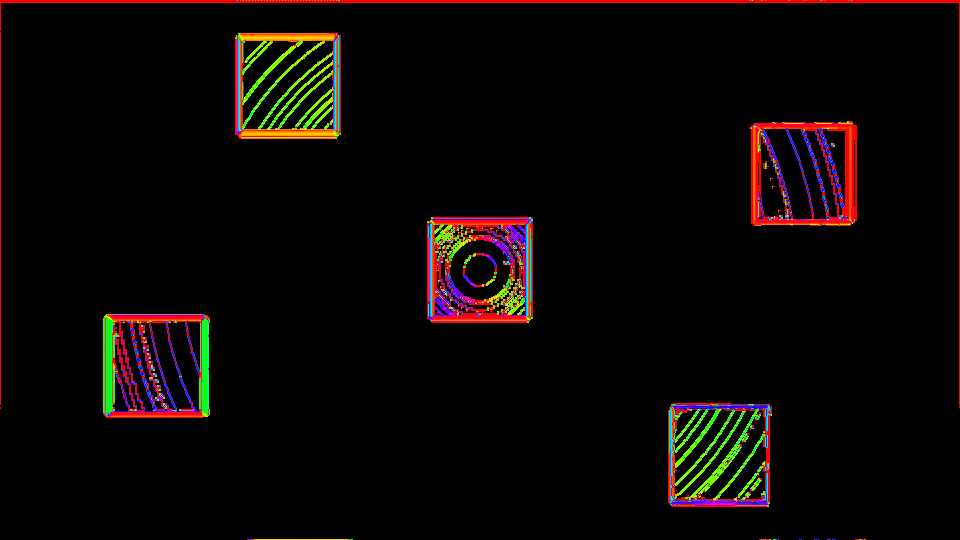
\includegraphics[width=0.5\textwidth]{img/final.png}}
    \caption{Mouvements visualisé avec une image HSL}
    \label{hsl}
\end{figure}

Une fois les mouvements détectés et exprimés pour chaque pixel, nous utilisons ces informations pour recréer
un flou de mouvement pour augmenter la sensation de fluidité de la vidéo.
Afin de réaliser cette illusion nous appliquons un flou directionnel sur chaque pixel de l'image en pondérant
sa valeurs avec ses voisins en fonction de la direction et de la taille de la norme~:

\[
%\begin{align}
	I'_{t} = \frac{1}{\sum^{k}_{i=0}\sum^{L}_{j=0}C_{u}(i,j)}
\]
\[
	\times \sum^{K}_{i=0}\sum^{L}_{j=0} C_{u}(i,j).I_{2n}(x+i-\frac{K}{2}, y+j-\frac{L}{2})
%\end{align}
\]

Où~:

\begin{itemize}
	\item $I$ est notre image en entrée 
	\item $I'$ est notre image en sortie 
	\item $C_{u}$ est le filtre de convolution de taille $K \times L$ associé au pixel $u$, centré en $u$
\end{itemize}

\subsection{Avantage et contraintes des méthodes}
\subsubsection{La décimation simple}
Les avantages substantiels de cette méthode sont : son temps d'exécution et sa simplicité. En effet, elle ne requiert guère plus de temps que l'ouverture du flux vidéo, le parcours d'une image sur deux et la fermeture du dit flux. Ce qui lui permet d'être très rapide mais en contre partie on doit payer le coût de n'effectuer aucun traitement sur les images ce qui peut provoquer une gêne à l'utilisateur lors de la visualisation de la séquence finale.

\subsubsection{La pondération simple}
La pondération simple requiert un temps d'exécution plus long mais cela reste modeste pour un traitement sur des vidéos dites \og FullHD \fg{} c'est à dire de résolution 1920x1080 pixels. Elle a pour avantage de pondérer deux images proches temporellement et donc possiblement spatialement en plus de de diminuer elle aussi le nombre d'images en sortie afin de pouvoir conserver une flux dit à 60 images par seconde.

Cependant cette méthode à faible coût ne prend en compte que la cohérence temporelle et ne cherche pas à recréer un vrai contenu natif 60 Hertz donc ne recrée pas de flou de mouvements. Le problème des saccades reste donc encore présent dans les vidéos de résultats.

\subsubsection{La double pondération}
Cette dernière technique de pondération repose sur un calcul à partir de 3 images consécutives. Elle a l'avantage de mieux prendre en compte le déplacement dans une scène grâce à la connaissance de l'image d'avant et celle d'après et réduit l'effet de saccades.

Mais elle ne prend toujours pas en compte la particularité du flou de mouvements des contenus à 60 images par seconde ni des vecteurs de déplacement entre deux images consécutives.

\subsubsection{Gradient spatio temporel}
Cette méthode est relativement plus coûteuse que les pondérations. En contre partie, elle s'appuie sur
l'approximation du flux optique des images pour recréer un flou de mouvement plus réaliste en prenant en
compte la direction et la vitesse du mouvement.

L'estimation du mouvement est par contre approximative, contrairement à un algorithme de type {\em Patch Match}.
Elle peut être mauvaise quand les mouvements sont de trop grande amplitude pour que les informations soit contenues dans 
le gradient spatio temporel --rappel: le gradient se base uniquement sur le pixel voisin de la frame précédente
ou suivante--. Malgré ce désavantage, cette technique propose un bon compromis entre les méthode de
pondération naïves et les méthodes précises mais très coûteuses basées sur {\em Patch Match}.

\subsection{Pourquoi les méthodes choisies permettent de répondre à la problématique}

\subsubsection{La décimation et les pondérations}
Ces méthodes dites \og Low Cost \fg{} permettent de répondre à la problématique car elles effectuent une décimation du nombre d'images dans la vidéo, ces traitements sont qualifiés de rapide compte tenu du type de séquences proposées en entrée. Il sera explicité dans la partie discussion que les vidéos obtenus avec ces méthodes donnent de bons résultats sur un public non averti.

\subsubsection{Le gradient spatio temporel}
Notre méthode basée sur le gradient spatio temporel permet aussi de décimer le nombre d'images de la vidéo. 
Ce traitement est plus lourd mais permet de meilleurs résultats visuels que les décimation et les pondérations
tout en fonctionnant en temps réel sur un processeur récent.

La difficultée reste l'estimation du mouvement dans la séquence,
une voie d'amélioration possible serait la construction un gradient tri-dimenssionel, 
tel que proposé dans l'article {\em Very high accuracy velocity estimation using orientation tensors, parametric motion, and simultaneous segmentation of the motion field}\cite{farneback2001}.
%------------------------------------------------

\section{Résultats et Discussion}
Suite aux développement de ces solutions nous avons pu constater que malgré leur qualifications \og Low Cost \fg{}, ces méthodes sont très performantes et donnent d'excellent résultats.

Pour interpréter ces résultats nous avons demandé à un panel d'utilisateurs de visionner la vidéo originale puis trois vidéos issus de ces méthodes naïves et de les classer selon quelques critères simples en nous donnant une note sur 4 (très mauvais, mauvais, bon et très bon).
\begin{center}

\begin{tabular}{|p{3cm}||c|c|c|}
  \hline
  \multicolumn{4}{|c|}{Résultats} \\
  \hline
  Vidéo & Saccades & Fluidité & Netteté\\ \hline
  Vidéo originale (FullHD 120Hz) & 4 & 4 & 4 \\ \hline
  Vidéo décimée & 1 & 2 & 4 \\ \hline
  Vidéo pondérée 50/50 & 2 & 4 & 2 \\ \hline
  Vidéo pondérée 25/50/25 & 4 & 4 & 2 \\ \hline
\end{tabular}

\end{center}

%------------------------------------------------

\section{Conclusion}
La problématique initiale de notre projet s'articulait autour des moyens possibles afin de pouvoir passer d'une vidéo de très haute qualité avec une cadence de 120 images par secondes (FullHD/4K 120IPS) à un contenu adapté pour d'anciennes générations de téléviseurs ou d'appareils mobiles ne permettant que d'afficher 60 images par secondes.
Nous devions développer des techniques aussi bien frugales telles qu'une simple décimation ou de la pondération, que plus gourmandes en termes de calculs et de temps d'exécution comme le gradient temporel ou plus rapides grâce à l'implémentation de calculs sur des processeurs de carte graphique.

On a pu voir grâce aux tests utilisateurs que malgré leur simplicité certaines des méthodes donnent de bons résultats en considérant le ratio qualité/temps de calcul. En particulier la double pondération, qui donne des résultats rapides et proches d'un contenu à 60 images par seconde natif.

Néanmoins il reste énormément de travail sur ce sujet si l'on veut un jour pouvoir efficacement adapter ce genre de contenu à la volée. Les méthodes proposées actuellement à \bcom cherchent à émuler un contenu 60Hz à partir d'une source à 120Hz. Les contenus actuels ne présentent pas les résultats d'une vrai vidéo enregistrée à une cadence d'image de 60Hz. C'est pour cela qu'il reste du travail à faire en terme de développement technique afin de se rapprocher le plus possible d'un contenu natif, légitime et authentique à 60Hz.

Cependant, si l'approximation est autorisée, comme semble le présenter les tests utilisateurs, les méthodes peu coûteuses en temps de calcul sont un bon compromis.
Le perfectionnement de notre méthode avec un gradient tridimensionnel offrirait ce type de résultats.
%------------------------------------------------
\phantomsection
\section*{Remerciements} % The \section*{} command stops section numbering

\addcontentsline{toc}{section}{Remerciements} % Adds this section to the table of contents

Nous voudrions remercier M. Jean-Yves AUBIE pour son indéfectible soutien ainsi que pour son temps mis à notre disposition lors des tests effectués à \bcom.\\

M. Olivier LE MEUR pour son aide apportée tout du long du projet et son temps passé avec nous.

%----------------------------------------------------------------------------------------
%	REFERENCE LIST
%----------------------------------------------------------------------------------------
\phantomsection
\bibliographystyle{unsrt}
\bibliography{references}

%----------------------------------------------------------------------------------------

\end{document}
